% Options for packages loaded elsewhere
\PassOptionsToPackage{unicode}{hyperref}
\PassOptionsToPackage{hyphens}{url}
%
\documentclass[
]{article}
\usepackage{lmodern}
\usepackage{amssymb,amsmath}
\usepackage{ifxetex,ifluatex}
\ifnum 0\ifxetex 1\fi\ifluatex 1\fi=0 % if pdftex
  \usepackage[T1]{fontenc}
  \usepackage[utf8]{inputenc}
  \usepackage{textcomp} % provide euro and other symbols
\else % if luatex or xetex
  \usepackage{unicode-math}
  \defaultfontfeatures{Scale=MatchLowercase}
  \defaultfontfeatures[\rmfamily]{Ligatures=TeX,Scale=1}
\fi
% Use upquote if available, for straight quotes in verbatim environments
\IfFileExists{upquote.sty}{\usepackage{upquote}}{}
\IfFileExists{microtype.sty}{% use microtype if available
  \usepackage[]{microtype}
  \UseMicrotypeSet[protrusion]{basicmath} % disable protrusion for tt fonts
}{}
\makeatletter
\@ifundefined{KOMAClassName}{% if non-KOMA class
  \IfFileExists{parskip.sty}{%
    \usepackage{parskip}
  }{% else
    \setlength{\parindent}{0pt}
    \setlength{\parskip}{6pt plus 2pt minus 1pt}}
}{% if KOMA class
  \KOMAoptions{parskip=half}}
\makeatother
\usepackage{xcolor}
\IfFileExists{xurl.sty}{\usepackage{xurl}}{} % add URL line breaks if available
\IfFileExists{bookmark.sty}{\usepackage{bookmark}}{\usepackage{hyperref}}
\hypersetup{
  pdftitle={data cleaning - vocab size},
  pdfauthor={Stephen Skalicky},
  hidelinks,
  pdfcreator={LaTeX via pandoc}}
\urlstyle{same} % disable monospaced font for URLs
\usepackage[margin=1in]{geometry}
\usepackage{color}
\usepackage{fancyvrb}
\newcommand{\VerbBar}{|}
\newcommand{\VERB}{\Verb[commandchars=\\\{\}]}
\DefineVerbatimEnvironment{Highlighting}{Verbatim}{commandchars=\\\{\}}
% Add ',fontsize=\small' for more characters per line
\usepackage{framed}
\definecolor{shadecolor}{RGB}{248,248,248}
\newenvironment{Shaded}{\begin{snugshade}}{\end{snugshade}}
\newcommand{\AlertTok}[1]{\textcolor[rgb]{0.94,0.16,0.16}{#1}}
\newcommand{\AnnotationTok}[1]{\textcolor[rgb]{0.56,0.35,0.01}{\textbf{\textit{#1}}}}
\newcommand{\AttributeTok}[1]{\textcolor[rgb]{0.77,0.63,0.00}{#1}}
\newcommand{\BaseNTok}[1]{\textcolor[rgb]{0.00,0.00,0.81}{#1}}
\newcommand{\BuiltInTok}[1]{#1}
\newcommand{\CharTok}[1]{\textcolor[rgb]{0.31,0.60,0.02}{#1}}
\newcommand{\CommentTok}[1]{\textcolor[rgb]{0.56,0.35,0.01}{\textit{#1}}}
\newcommand{\CommentVarTok}[1]{\textcolor[rgb]{0.56,0.35,0.01}{\textbf{\textit{#1}}}}
\newcommand{\ConstantTok}[1]{\textcolor[rgb]{0.00,0.00,0.00}{#1}}
\newcommand{\ControlFlowTok}[1]{\textcolor[rgb]{0.13,0.29,0.53}{\textbf{#1}}}
\newcommand{\DataTypeTok}[1]{\textcolor[rgb]{0.13,0.29,0.53}{#1}}
\newcommand{\DecValTok}[1]{\textcolor[rgb]{0.00,0.00,0.81}{#1}}
\newcommand{\DocumentationTok}[1]{\textcolor[rgb]{0.56,0.35,0.01}{\textbf{\textit{#1}}}}
\newcommand{\ErrorTok}[1]{\textcolor[rgb]{0.64,0.00,0.00}{\textbf{#1}}}
\newcommand{\ExtensionTok}[1]{#1}
\newcommand{\FloatTok}[1]{\textcolor[rgb]{0.00,0.00,0.81}{#1}}
\newcommand{\FunctionTok}[1]{\textcolor[rgb]{0.00,0.00,0.00}{#1}}
\newcommand{\ImportTok}[1]{#1}
\newcommand{\InformationTok}[1]{\textcolor[rgb]{0.56,0.35,0.01}{\textbf{\textit{#1}}}}
\newcommand{\KeywordTok}[1]{\textcolor[rgb]{0.13,0.29,0.53}{\textbf{#1}}}
\newcommand{\NormalTok}[1]{#1}
\newcommand{\OperatorTok}[1]{\textcolor[rgb]{0.81,0.36,0.00}{\textbf{#1}}}
\newcommand{\OtherTok}[1]{\textcolor[rgb]{0.56,0.35,0.01}{#1}}
\newcommand{\PreprocessorTok}[1]{\textcolor[rgb]{0.56,0.35,0.01}{\textit{#1}}}
\newcommand{\RegionMarkerTok}[1]{#1}
\newcommand{\SpecialCharTok}[1]{\textcolor[rgb]{0.00,0.00,0.00}{#1}}
\newcommand{\SpecialStringTok}[1]{\textcolor[rgb]{0.31,0.60,0.02}{#1}}
\newcommand{\StringTok}[1]{\textcolor[rgb]{0.31,0.60,0.02}{#1}}
\newcommand{\VariableTok}[1]{\textcolor[rgb]{0.00,0.00,0.00}{#1}}
\newcommand{\VerbatimStringTok}[1]{\textcolor[rgb]{0.31,0.60,0.02}{#1}}
\newcommand{\WarningTok}[1]{\textcolor[rgb]{0.56,0.35,0.01}{\textbf{\textit{#1}}}}
\usepackage{graphicx,grffile}
\makeatletter
\def\maxwidth{\ifdim\Gin@nat@width>\linewidth\linewidth\else\Gin@nat@width\fi}
\def\maxheight{\ifdim\Gin@nat@height>\textheight\textheight\else\Gin@nat@height\fi}
\makeatother
% Scale images if necessary, so that they will not overflow the page
% margins by default, and it is still possible to overwrite the defaults
% using explicit options in \includegraphics[width, height, ...]{}
\setkeys{Gin}{width=\maxwidth,height=\maxheight,keepaspectratio}
% Set default figure placement to htbp
\makeatletter
\def\fps@figure{htbp}
\makeatother
\setlength{\emergencystretch}{3em} % prevent overfull lines
\providecommand{\tightlist}{%
  \setlength{\itemsep}{0pt}\setlength{\parskip}{0pt}}
\setcounter{secnumdepth}{-\maxdimen} % remove section numbering

\title{data cleaning - vocab size}
\author{Stephen Skalicky}
\date{22/09/2021}

\begin{document}
\maketitle

\hypertarget{thanks-to-tj-for-providing-the-data-and-guiding-us-through-the-discussion}{%
\subsubsection{Thanks to TJ for providing the data and guiding us
through the
discussion!}\label{thanks-to-tj-for-providing-the-data-and-guiding-us-through-the-discussion}}

The goal of this lesson is to practice data wrangling and exploration
with less scaffolding. TJ has provided a data set and what that final
data set should look like.

\hypertarget{loading-and-observing-the-dataset}{%
\subsection{Loading and observing the
dataset}\label{loading-and-observing-the-dataset}}

More often than not, raw data looks very different to data that appears
in a publication. This means that a lot of time is spent cleaning the
data. In this exercise, we will practice the process of cleaning up
data. The first thing we need to do is import the data and look at it.

You can download the data from
\href{https://www.stephenskalicky.com/r_data/testData.csv}{here}.\\

Or you can pass the URL directly to \texttt{read\_csv} to get the data
into R.

\begin{Shaded}
\begin{Highlighting}[]
\NormalTok{dat <-}\StringTok{ }\KeywordTok{read_csv}\NormalTok{(}\StringTok{'https://www.stephenskalicky.com/r_data/testData.csv'}\NormalTok{)}
\end{Highlighting}
\end{Shaded}

\begin{verbatim}
## 
## -- Column specification --------------------------------------------------------
## cols(
##   .default = col_double()
## )
## ℹ Use `spec()` for the full column specifications.
\end{verbatim}

Examine the data. What does each row represent? What are the column
names?

\hypertarget{main-task}{%
\section{Main task}\label{main-task}}

\hypertarget{what-is-the-score-for-each-participant-and-what-is-their-vocabulary-size}{%
\subsection{\texorpdfstring{What is the score for each participant, and
what is their vocabulary size?\\
}{What is the score for each participant, and what is their vocabulary size? }}\label{what-is-the-score-for-each-participant-and-what-is-their-vocabulary-size}}

In order to answer these questions we need to do a variety of things.\\

In the session, we decided it would be fun to compare and contrast the
tidyverse and base r methods to answer these questions. The objects with
\texttt{tv} at the end are the tidyverse methods, while the objects with
\texttt{b} at the end are base R.

\hypertarget{the-first-task-is-to-get-only-the-vst-data-dont-need-anything-related-to-levels-age-etc..}{%
\subsubsection{the first task is to get only the VST data (don't need
anything related to levels, age,
etc.).}\label{the-first-task-is-to-get-only-the-vst-data-dont-need-anything-related-to-levels-age-etc..}}

\begin{Shaded}
\begin{Highlighting}[]
\CommentTok{# subset VST data (so we want ID + all of the columns with vst.qX in the name)}

\CommentTok{# pipe using tidyverse}
\NormalTok{vst_data_tv <-}\StringTok{ }\NormalTok{dat }\OperatorTok
\StringTok{  }\NormalTok{dplyr}\OperatorTok{::}\KeywordTok{select}\NormalTok{(}\KeywordTok{c}\NormalTok{(ID, }\KeywordTok{contains}\NormalTok{(}\StringTok{'vst.'}\NormalTok{)))}

\CommentTok{# subset function from base R}
\NormalTok{vst_data_b <-}\StringTok{ }\KeywordTok{subset}\NormalTok{(dat, }\DataTypeTok{select =} \KeywordTok{grep}\NormalTok{(}\StringTok{"ID|vst."}\NormalTok{, }\KeywordTok{names}\NormalTok{(dat), }\DataTypeTok{value =}\NormalTok{ T))}

\KeywordTok{identical}\NormalTok{(vst_data_tv, vst_data_b)}
\end{Highlighting}
\end{Shaded}

\begin{verbatim}
## [1] TRUE
\end{verbatim}

\hypertarget{the-next-task-is-to-remove-anyone-who-has-na-for-a-vst-test}{%
\subsubsection{the next task is to remove anyone who has NA for a vst
test}\label{the-next-task-is-to-remove-anyone-who-has-na-for-a-vst-test}}

\begin{Shaded}
\begin{Highlighting}[]
\CommentTok{# remove NAs (n should = 16) (any row that has an NA anywhere)}

\CommentTok{# Tidyverse will drop a row where ANY column has an NA}
\NormalTok{vst_data_tv1 <-}\StringTok{ }\NormalTok{vst_data_tv }\OperatorTok
\StringTok{  }\KeywordTok{drop_na}\NormalTok{(vst.q1)}

\CommentTok{# Slicing with Base R - looking for NA in the second column only}
\CommentTok{# Slicing is a technique used by other programming language (with different syntax) - so it can be a useful method but harder to read}
\NormalTok{vst_data_b1 <-}\StringTok{ }\NormalTok{vst_data_b[}\OperatorTok{!}\KeywordTok{is.na}\NormalTok{(vst_data_b[,}\DecValTok{2}\NormalTok{]),]}
\end{Highlighting}
\end{Shaded}

\hypertarget{in-case-you-want-to-go-through-some-potentially-redundant-steps-here-they-are}{%
\subsubsection{in case you want to go through some potentially redundant
steps here they
are}\label{in-case-you-want-to-go-through-some-potentially-redundant-steps-here-they-are}}

\texttt{compute\ sums\ for\ each\ ten\ questions\ that\ make\ up\ a\ 1k\ freq\ band}
\texttt{rename\ datvst\_summed\_by\_level\textquotesingle{}s\ columns\ to\ appropriate\ names}

\hypertarget{the-next-step-is-to-create-a-tabledftibble-with-three-columns-person-total-score-vst-and-total-vocabulary-vsize}{%
\subsubsection{the next step is to create a table/df/tibble with three
columns: person, total score (VST), and total vocabulary
(Vsize)}\label{the-next-step-is-to-create-a-tabledftibble-with-three-columns-person-total-score-vst-and-total-vocabulary-vsize}}

\begin{Shaded}
\begin{Highlighting}[]
\CommentTok{# create a table of person, total score, total vocab size}
\CommentTok{# the vst ranges from 0 - 100. let's calculate each subject's score on the vst.}


\CommentTok{# tidyverse method one}
\NormalTok{vst_data_tv2 <-}\StringTok{ }\NormalTok{vst_data_tv1 }\OperatorTok
\StringTok{  }\KeywordTok{rowwise}\NormalTok{(ID) }\OperatorTok\StringTok{ }
\StringTok{  }\KeywordTok{mutate}\NormalTok{(}\DataTypeTok{VST =} \KeywordTok{sum}\NormalTok{(}\KeywordTok{c_across}\NormalTok{(}\KeywordTok{contains}\NormalTok{(}\StringTok{'vst'}\NormalTok{))))}

\CommentTok{# tidyverse method two (via Micky Vale)}
\NormalTok{vst_data_tv2 <-}\StringTok{ }\NormalTok{vst_data_tv1 }\OperatorTok
\StringTok{    }\KeywordTok{mutate}\NormalTok{(}\DataTypeTok{VST =} \KeywordTok{rowSums}\NormalTok{(}\KeywordTok{select}\NormalTok{(., }\KeywordTok{contains}\NormalTok{(}\StringTok{'vst'}\NormalTok{))))}

\CommentTok{# glue it into a df. }
\NormalTok{finalResults_tv <-}\StringTok{ }\KeywordTok{tibble}\NormalTok{(}\DataTypeTok{person =}\NormalTok{ vst_data_tv1}\OperatorTok{$}\NormalTok{ID, }\DataTypeTok{VST =}\NormalTok{ vst_data_tv2}\OperatorTok{$}\NormalTok{VST)}
  
\CommentTok{# baseRisbestR}
\CommentTok{# will need to use apply here because this needs to be done row-wise (i think?)}
\NormalTok{vst_data_b2 <-}\StringTok{ }\KeywordTok{apply}\NormalTok{(vst_data_b1[,}\DecValTok{2}\OperatorTok{:}\KeywordTok{ncol}\NormalTok{(vst_data_b1)], }\DecValTok{1}\NormalTok{, sum)}

\NormalTok{finalResults_b <-}\StringTok{ }\KeywordTok{data.frame}\NormalTok{(}\DataTypeTok{person =}\NormalTok{ vst_data_b1}\OperatorTok{$}\NormalTok{ID, }\DataTypeTok{VST =}\NormalTok{ vst_data_b2)}


\NormalTok{finalResults_b <-}\StringTok{ }\KeywordTok{data.frame}\NormalTok{(}\DataTypeTok{person =}\NormalTok{ vst_data_b1}\OperatorTok{$}\NormalTok{ID, }\DataTypeTok{VST =}\NormalTok{ vst_data_b2, }\DataTypeTok{Vsize =}\NormalTok{ vst_data_b2}\OperatorTok{*}\DecValTok{200}\NormalTok{)}
\end{Highlighting}
\end{Shaded}

\begin{Shaded}
\begin{Highlighting}[]
\NormalTok{finalResults2 <-}\StringTok{ }\NormalTok{vst_data_tv1 }\OperatorTok
\StringTok{     }\KeywordTok{mutate}\NormalTok{(}\DataTypeTok{person =}\NormalTok{ ID, }\DataTypeTok{VST =} \KeywordTok{rowSums}\NormalTok{ (}\KeywordTok{select}\NormalTok{(., }\KeywordTok{contains}\NormalTok{ (}\StringTok{'vst'}\NormalTok{))), }\DataTypeTok{Vsize =}\NormalTok{ VST }\OperatorTok{*}\StringTok{ }\DecValTok{200}\NormalTok{) }\OperatorTok
\StringTok{     }\KeywordTok{select}\NormalTok{(person, VST, Vsize)}
\end{Highlighting}
\end{Shaded}

\hypertarget{add-vsize-this-is-also-done-above---we-adjusted-the-above-code-after-doing-the-below.-this-shows-you-that-vsize-was-just-vst200.}{%
\subsubsection{add Vsize (this is also done above - we adjusted the
above code after doing the below). This shows you that Vsize was just
VST*200.}\label{add-vsize-this-is-also-done-above---we-adjusted-the-above-code-after-doing-the-below.-this-shows-you-that-vsize-was-just-vst200.}}

\begin{Shaded}
\begin{Highlighting}[]
\CommentTok{# add one more column which is vsize}
\CommentTok{# what is vsize? Well, it looks like each correct answer is indicative of 200 words or something like that}
\CommentTok{# so we can easily create a new column by multiplying VST*200}

\CommentTok{# we can actually use mutate here...}
\NormalTok{finalResults_tv <-}\StringTok{ }\NormalTok{finalResults_tv }\OperatorTok
\StringTok{  }\KeywordTok{mutate}\NormalTok{(}\DataTypeTok{Vsize =}\NormalTok{ VST }\OperatorTok{*}\StringTok{ }\DecValTok{200}\NormalTok{)}

\CommentTok{# what about base R? }
\NormalTok{finalResults_b[}\StringTok{'Vsize'}\NormalTok{] <-}\StringTok{ }\NormalTok{finalResults_b}\OperatorTok{$}\NormalTok{VST}\OperatorTok{*}\DecValTok{200}
\CommentTok{# this is probably a better way to to do it this way}
\NormalTok{finalResults_b}\OperatorTok{$}\NormalTok{Vsize <-}\StringTok{ }\NormalTok{finalResults_b[,}\StringTok{'VST'}\NormalTok{] }\OperatorTok{*}\StringTok{ }\DecValTok{200}
\end{Highlighting}
\end{Shaded}

\hypertarget{plots-for-fun}{%
\subsubsection{plots for fun}\label{plots-for-fun}}

\begin{Shaded}
\begin{Highlighting}[]
\KeywordTok{ggplot}\NormalTok{(finalResults_b, }\KeywordTok{aes}\NormalTok{(}\DataTypeTok{x =}\NormalTok{ VST, }\DataTypeTok{y =}\NormalTok{ Vsize)) }\OperatorTok{+}
\StringTok{  }\CommentTok{#geom_point() + }
\StringTok{  }\KeywordTok{geom_text}\NormalTok{(}\KeywordTok{aes}\NormalTok{(}\DataTypeTok{label =}\NormalTok{ person))}
\end{Highlighting}
\end{Shaded}

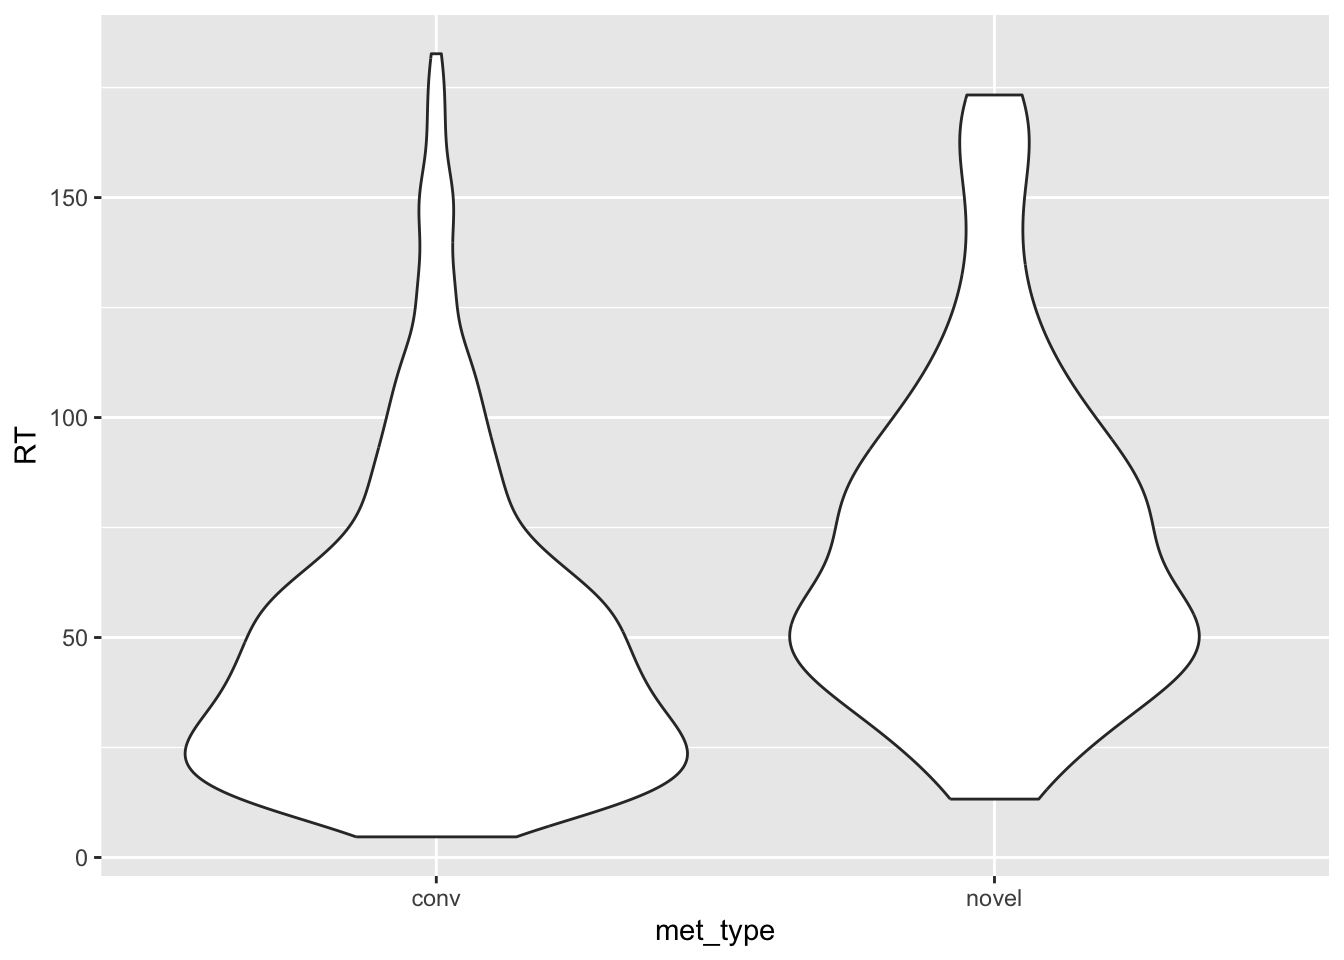
\includegraphics{vst-cleaning_files/figure-latex/unnamed-chunk-8-1.pdf}

\hypertarget{your-final-dataframe-should-look-like-this}{%
\subsection{Your final dataframe should look like
this:}\label{your-final-dataframe-should-look-like-this}}

\begin{verbatim}
person  VST     Vsize
01         79     15800
02         85     17000
03         78     15600
04         73     14600
05         85     17000
06         90     18000
07         93     18600
08         68     13600
09         78     15600
10         82     16400
11         77     15400
12         56     11200
13         93     18600
14         72     14400
15         63     12600
16         92     18400
\end{verbatim}

\end{document}
